% ! TeX program = xelatex
\documentclass[12pt]{beamer}
\usetheme{metropolis}
\usepackage{tabularx}
\usepackage{changepage}
\usepackage{float}
\usepackage{ragged2e}
\usepackage{amsmath}
\usepackage{graphicx}
\usepackage{appendix}
\usepackage[round]{natbib}   % omit 'round' option if you prefer square brackets
\bibliographystyle{aer}

\usepackage{xeCJK}
\setCJKmainfont{regular}[
    Path="../fonts/simplified_chinese/noto_serif/",
    BoldFont=bold.otf
]
\xeCJKDeclareSubCJKBlock{Hangul}{"1100 -> "11FF, "3130 -> "318F, "A960 -> "A97F, "AC00 -> "D7AF, "D7B0 -> "D7FF}
\setCJKmainfont{regular}[
    Hangul,
    Path="../fonts/korean/noto_serif/",
    BoldFont=bold.otf
]

\xeCJKDeclareSubCJKBlock{Kana}{"3040 -> "309F, "30A0 -> "30FF, "31F0 -> "31FF, "1B000 -> "1B0FF}
\setCJKmainfont{regular}[
    Kana,
    Path="../fonts/japanese/noto_serif/",
    BoldFont=bold.otf
]



\title{\huge{Auto-EPU}}
\author{Hsiu-Hsuan(Jacky) Yeh}
\date{2024-02-19}
\begin{document}
\maketitle


\begin{frame}{Outline}
\tableofcontents
\end{frame}


\section{Chat With PDF}


\begin{frame}{ChatGPT-4}
    Upload the QJE version of the paper, \cite{Baker2016}


You are a Taiwanese Economist and plan to construct the EPU index of Taiwan.
Define keywords in each E, P, U set

Assistant:

\begin{table}[H]
\renewcommand\arraystretch{1.2}
% \caption{}
% \label{Taiwan policy keywords}
\begin{adjustwidth}{-0.1cm}{}
\begin{center}
\setlength{\tabcolsep}{30pt}
{
    \fontsize{10}{10} \selectfont
    {
\def\sym#1{\ifmmode^{#1}\else\(^{#1}\)\fi}
\begin{tabular}{l c c}
\hline\hline

\multicolumn{1}{c}{(1)}
&\multicolumn{1}{c}{(2)}
&\multicolumn{1}{c}{(3)}
\\

\multicolumn{1}{c}{Economy}
&\multicolumn{1}{c}{Policy}
&\multicolumn{1}{c}{Uncertainty}
\\
\hline
經濟              & 政策             & 不確定                  \\
成長               & 法規             & 風險                    \\
發展              & 立法             & 擔憂                    \\
投資               & 財政             & 不穩定                  \\
消費              & 金融             & 變數                    \\
生產              & 稅務             &                         \\
貿易              & 預算             &                         \\
\hline\hline
\end{tabular}
}

}
\end{center}
\end{adjustwidth}
% \begin{justify}
% {\tiny
%     Note:
% }
% \end{justify}
\end{table}
\end{frame}


\begin{frame}{Cluade.ai-beta}
Note: only use the first 25 page of pdf from QJE
\begin{table}[H]
\renewcommand\arraystretch{1.2}
% \caption{}
% \label{Taiwan policy keywords}
\begin{adjustwidth}{-0.1cm}{}
\begin{center}
\setlength{\tabcolsep}{30pt}
{
    \fontsize{10}{10} \selectfont
    {
\def\sym#1{\ifmmode^{#1}\else\(^{#1}\)\fi}
\begin{tabular}{l c c c}
\hline\hline

\multicolumn{1}{c}{(1)}
&\multicolumn{1}{c}{(2)}
&\multicolumn{1}{c}{(3)}
&\multicolumn{1}{c}{(4)}
\\

\multicolumn{1}{c}{country}
&\multicolumn{1}{c}{vote}
&\multicolumn{1}{c}{definition}
&\multicolumn{1}{c}{definition with SC}
\\
\hline
TW & 8.571429 & 8.571429 & 17.142857 \\
CN & 12.903226 & 9.677419 & 16.129032 \\
JP & 6.250000 & 9.375000 & 12.500000 \\
KR & 17.391304 & 13.043478 & 13.043478 \\
US & 25.000000 & 37.500000 & 50.000000 \\
AU & 23.076923 & 15.384615 & 23.076923 \\
\hline\hline
\end{tabular}
}

}
\end{center}
\end{adjustwidth}
% \begin{justify}
% {\tiny
%     Note:
% }
% \end{justify}
\end{table}
\end{frame}


\section{Generation Analysis of Self-Consistency}


\subsection{Word Cloud}
\begin{frame}{Economy Category, ChatGPT-3.5}
\begin{figure}[H]
% \caption{Economy Category}
\centering
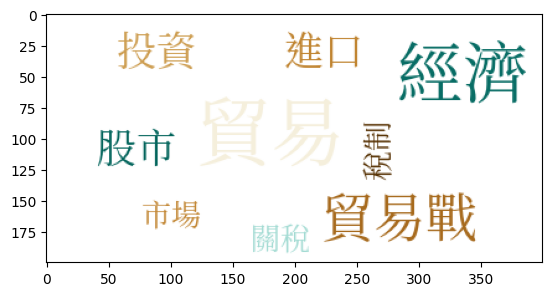
\includegraphics[width=11.5cm]{Figures/fig1.png}
\end{figure}
\end{frame}


\begin{frame}{Economy Category, ChatGPT-4}
\begin{figure}[H]
% \caption{Economy Category}
\centering
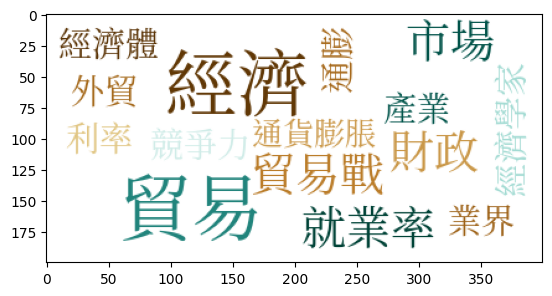
\includegraphics[width=11.5cm]{Figures/fig2.png}
\end{figure}
\end{frame}


\begin{frame}{Economy Category, Claude.ai-beta}
\begin{figure}[H]
% \caption{Economy Category}
\centering
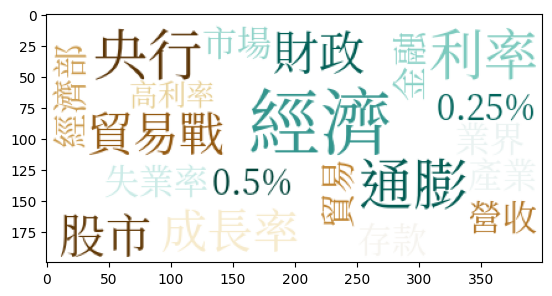
\includegraphics[width=11.5cm]{Figures/fig3.png}
\end{figure}
\end{frame}


\begin{frame}{Policy Category, ChatGPT-3.5}
\begin{figure}[H]
% \caption{Economy Category}
\centering
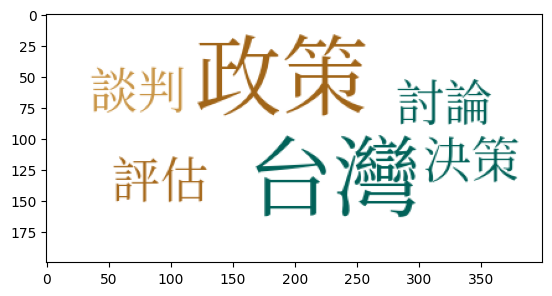
\includegraphics[width=11.5cm]{Figures/fig4.png}
\end{figure}
\end{frame}


\begin{frame}{Policy Category, ChatGPT-4}
\begin{figure}[H]
% \caption{Economy Category}
\centering
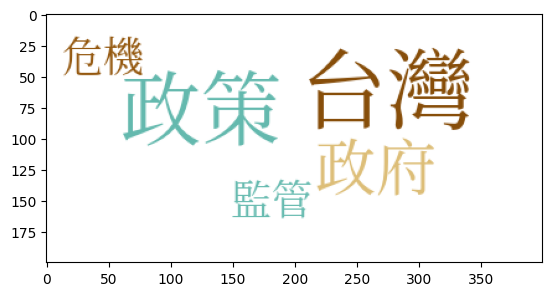
\includegraphics[width=11.5cm]{Figures/fig5.png}
\end{figure}
\end{frame}


\begin{frame}{Policy Category, Claude.ai-beta}
\begin{figure}[H]
% \caption{Economy Category}
\centering
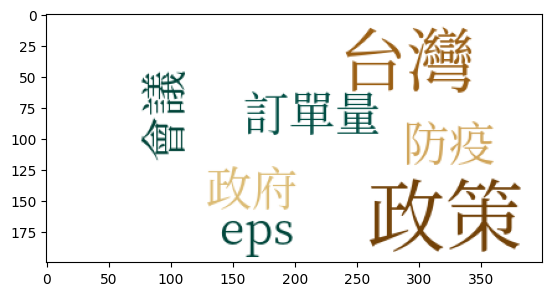
\includegraphics[width=11.5cm]{Figures/fig6.png}
\end{figure}
\end{frame}


\begin{frame}{Uncertainty Category, ChatGPT-3.5}
\begin{figure}[H]
% \caption{Economy Category}
\centering
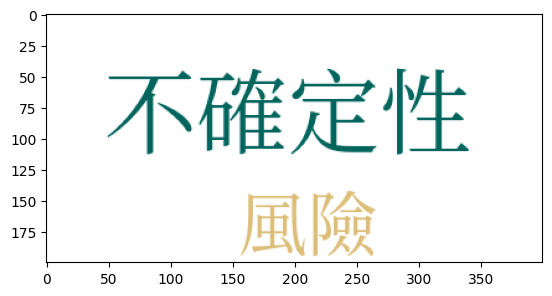
\includegraphics[width=11.5cm]{Figures/fig7.png}
\end{figure}
\end{frame}


\begin{frame}{Uncertainty Category, ChatGPT-4}
\begin{figure}[H]
% \caption{Economy Category}
\centering
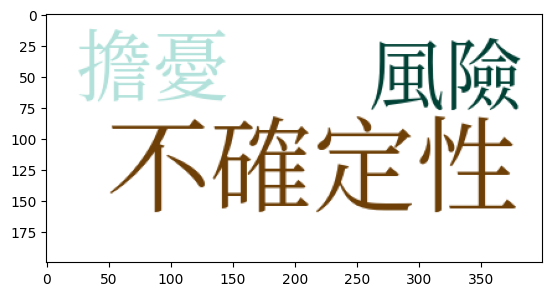
\includegraphics[width=11.5cm]{Figures/fig8.png}
\end{figure}
\end{frame}


\begin{frame}{Uncertainty Category, Claude.ai-beta}
\begin{figure}[H]
% \caption{Economy Category}
\centering
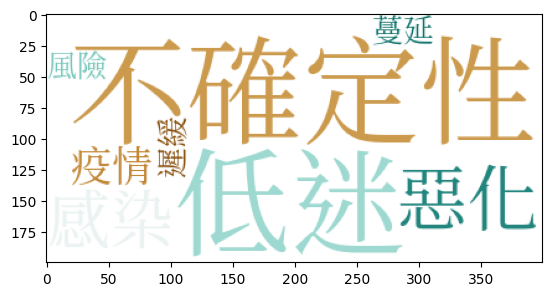
\includegraphics[width=11.5cm]{Figures/fig9.png}
\end{figure}
\end{frame}


\subsection{Accuracy}
\begin{frame}{Accuracy}
\begin{figure}[H]
% \caption{Economy Category}
\centering
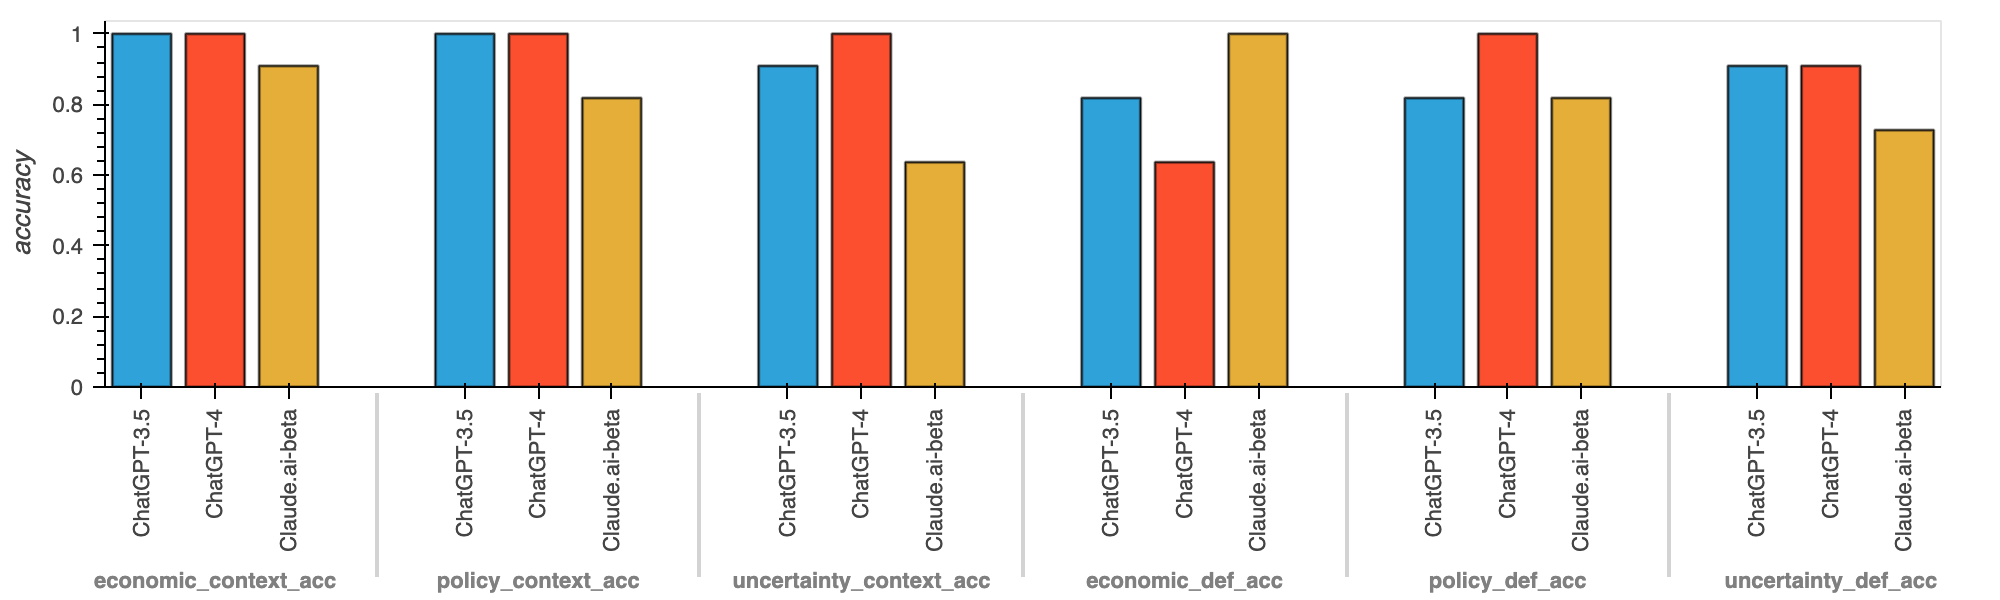
\includegraphics[width=11.5cm]{Figures/fig10.png}
\end{figure}
\end{frame}


\section{Prompt For Different Categories/Paradigms}


\begin{frame}
\end{frame}


\begin{frame}{Categories}
\begin{itemize}
    \item Economy
    \begin{itemize}
        \item the most common vocabularies that are related to economy
    \end{itemize}
    \item Policy
    \begin{itemize}
        \item the most common vocabularies that are related to policy
    \end{itemize}
    \item Uncertainty
    \begin{itemize}
        \item the most common vocabularies describing economic-relevant
            uncertainty
    \end{itemize}
\end{itemize}
\end{frame}


\begin{frame}{Categoty-Level Paradigms}
\begin{itemize}
    \item talent
    \item newspaper copora
    \begin{itemize}
        \item newspaper reader
        \item newspaper editor
        \item economist
    \end{itemize}
    \item add definition
    \item definition with SC
\end{itemize}
\end{frame}



\begin{frame}{Policy Relation}
\begin{enumerate}
    \item synonymous vocabularies which are nouns and related to "policy"
    \item "government occupations" which are highly related to "national policy"
    \item "government agency" which are highly related to "national policy"
    \item synonymous vocabularies which are verbs and related to "policy"
\end{enumerate}
\end{frame}


\section{Query Analysis}


\subsection{Entropy}
\begin{frame}{Policy Entropy, Among Models}
\begin{figure}[H]
% \caption{Economy Category}
\centering
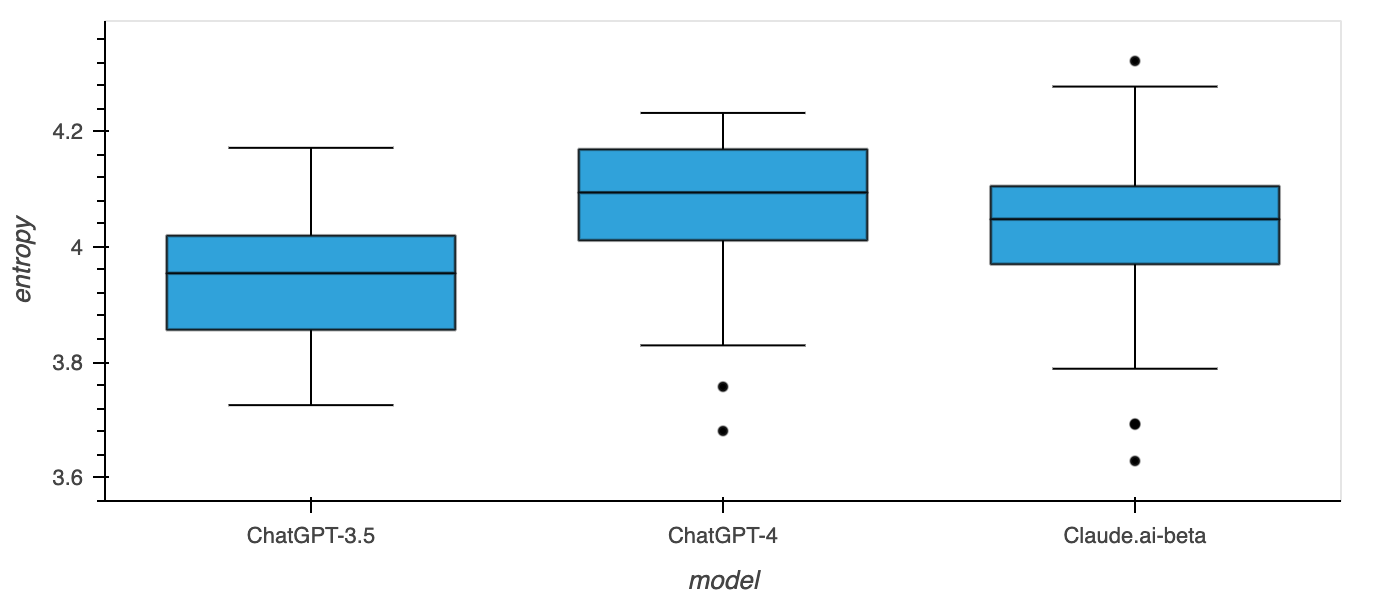
\includegraphics[width=11.5cm]{Figures/fig11.png}
\end{figure}
\end{frame}


\begin{frame}{Policy Entropy, Among Paradigms}
\begin{figure}[H]
% \caption{Economy Category}
\centering
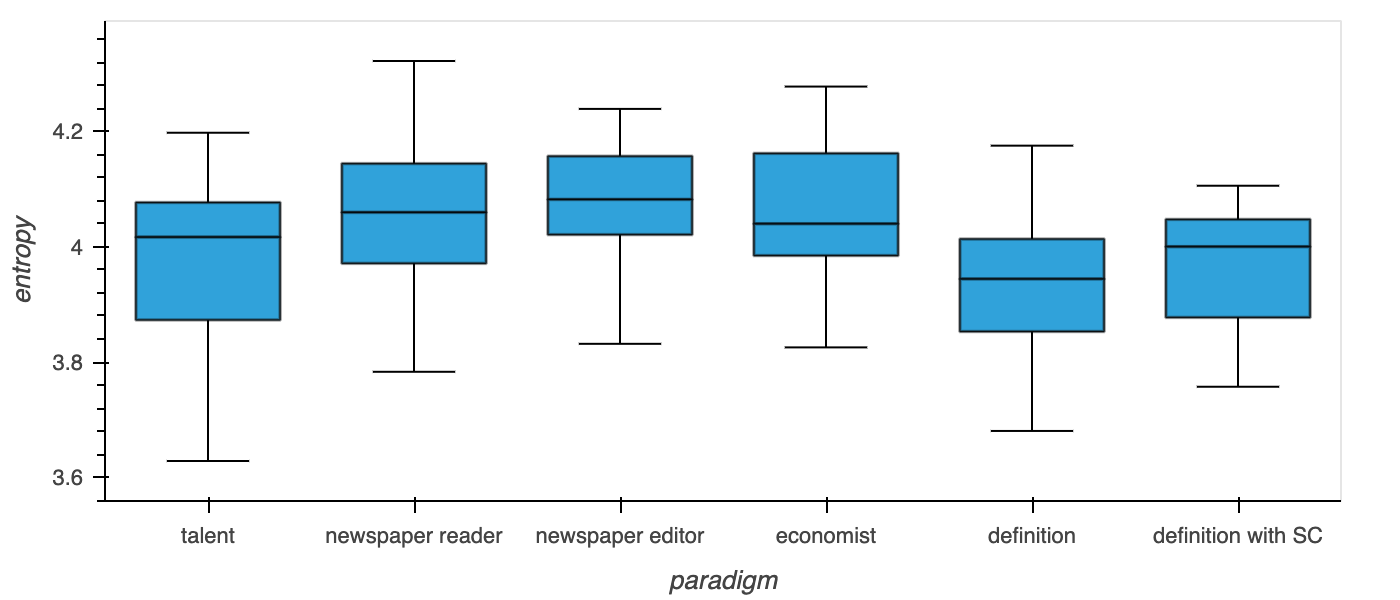
\includegraphics[width=11.5cm]{Figures/fig12.png}
\end{figure}
\end{frame}


\begin{frame}{Uncertainty Entropy, Among Models}
\begin{figure}[H]
% \caption{Economy Category}
\centering
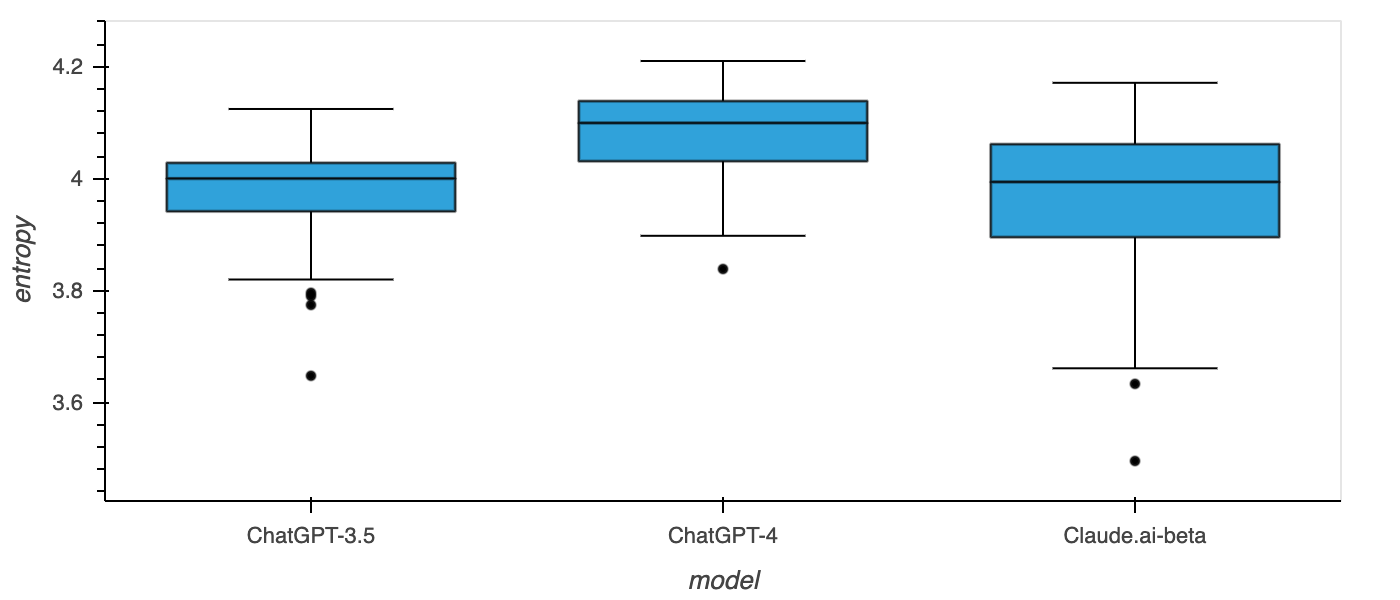
\includegraphics[width=11.5cm]{Figures/fig13.png}
\end{figure}
\end{frame}


\begin{frame}{Uncertainty Entropy, Among Paradigms}
\begin{figure}[H]
% \caption{Economy Category}
\centering
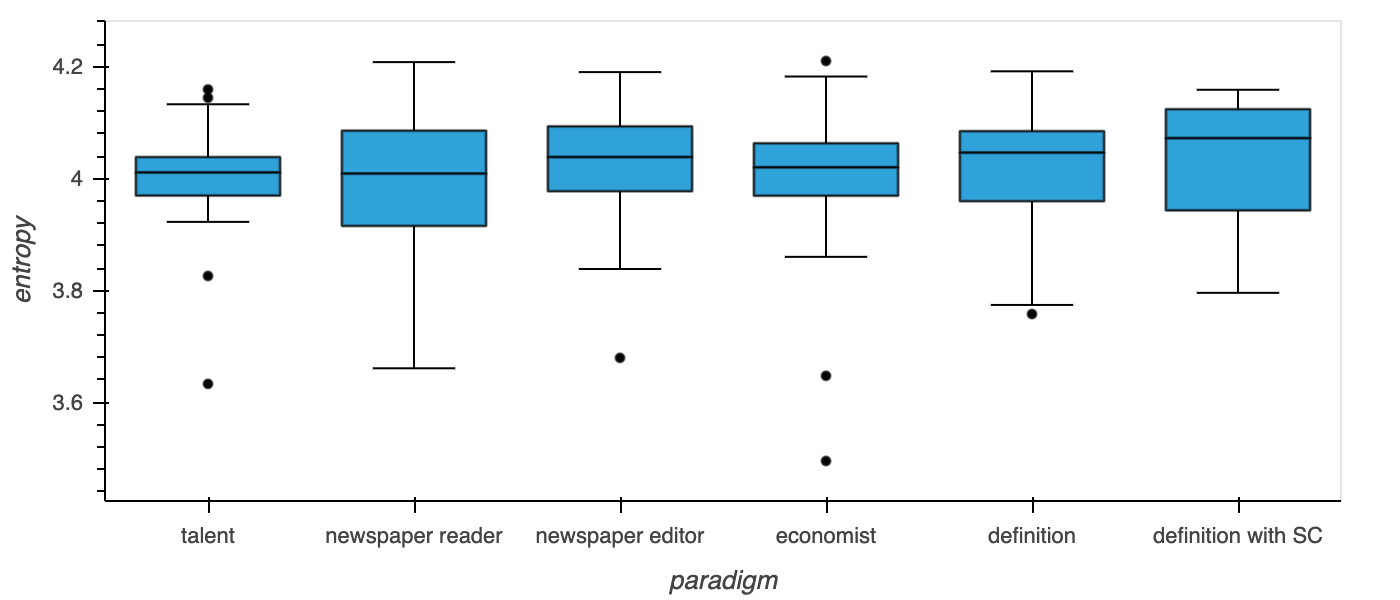
\includegraphics[width=11.5cm]{Figures/fig14.png}
\end{figure}
\end{frame}


\begin{frame}{Entropy Of Policy Relation 1, Among Models}
\begin{figure}[H]
% \caption{Economy Category}
\centering
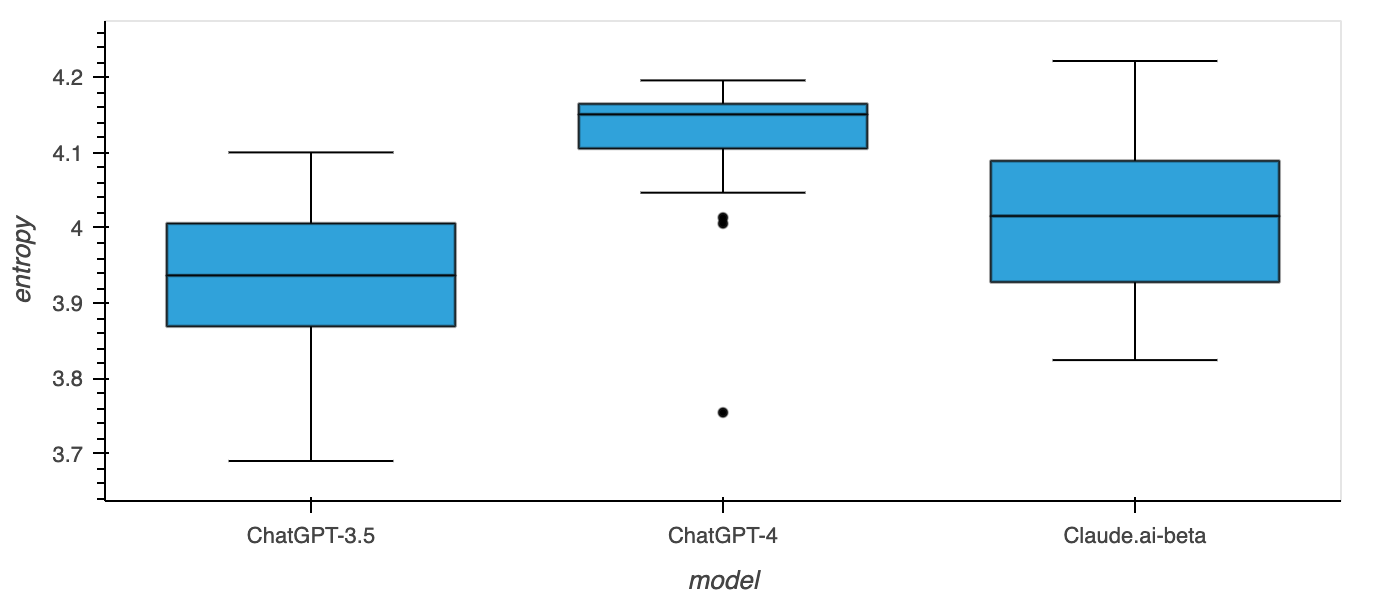
\includegraphics[width=11.5cm]{Figures/fig15.png}
\end{figure}
\end{frame}


\begin{frame}{Entropy Of Policy Relation 1, Among Paradigms}
\begin{figure}[H]
% \caption{Economy Category}
\centering
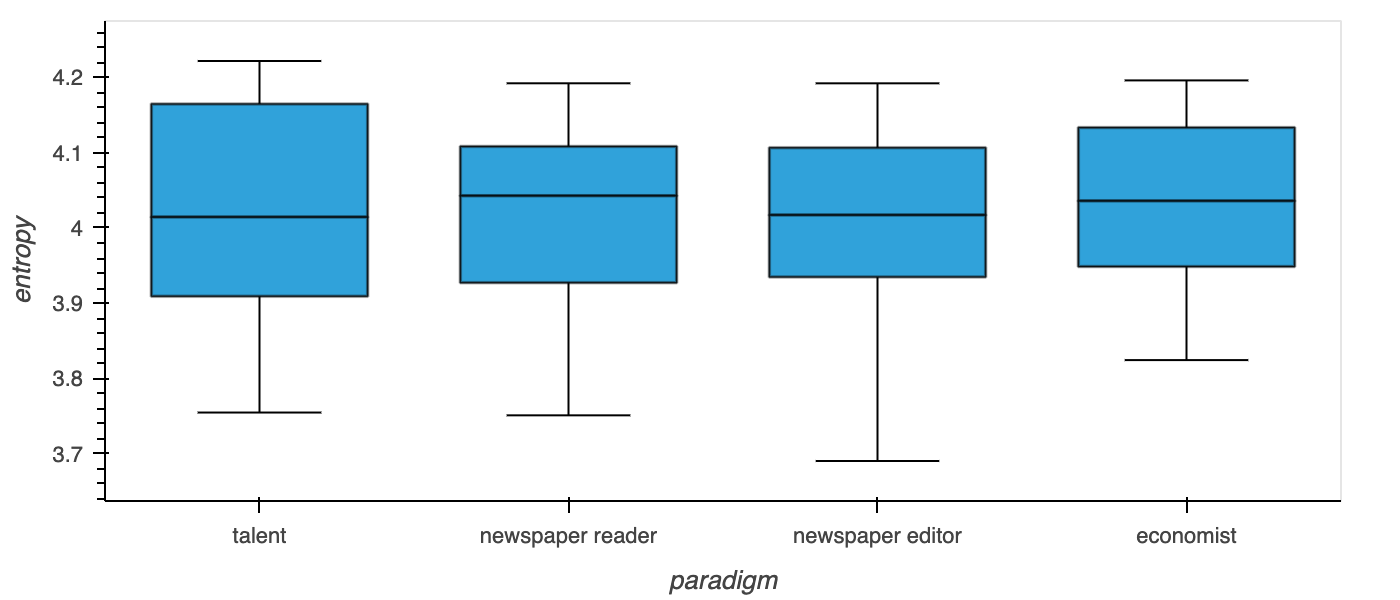
\includegraphics[width=11.5cm]{Figures/fig16.png}
\end{figure}
\end{frame}


\begin{frame}{Entropy Of Policy Relation 2, Among Models}
\begin{figure}[H]
% \caption{Economy Category}
\centering
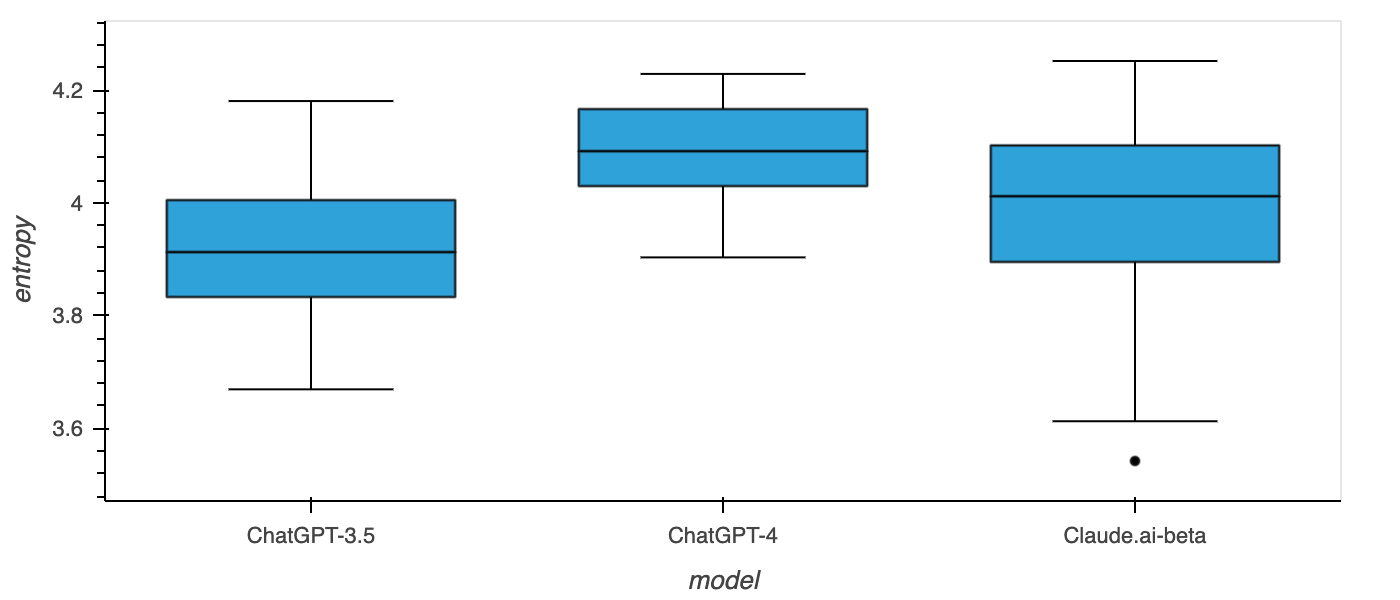
\includegraphics[width=11.5cm]{Figures/fig17.png}
\end{figure}
\end{frame}


\begin{frame}{Entropy Of Policy Relation 2, Among Paradigms}
\begin{figure}[H]
% \caption{Economy Category}
\centering
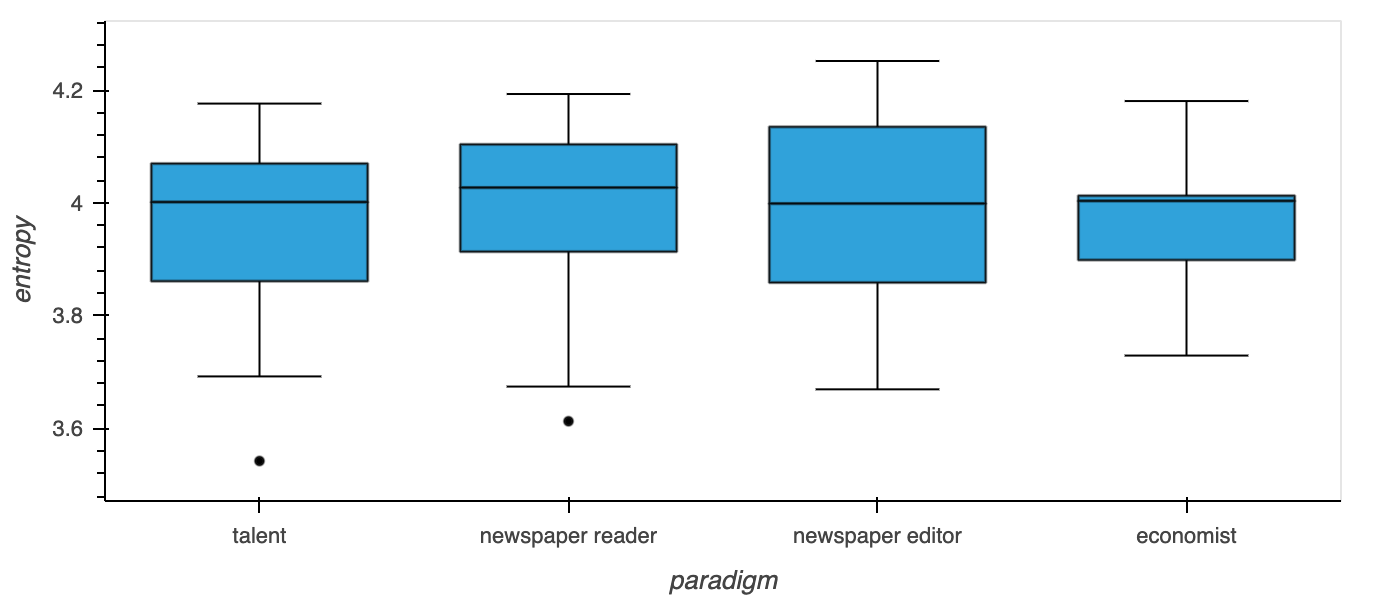
\includegraphics[width=11.5cm]{Figures/fig18.png}
\end{figure}
\end{frame}


\begin{frame}{Entropy Of Policy Relation 3, Among Models}
\begin{figure}[H]
% \caption{Economy Category}
\centering
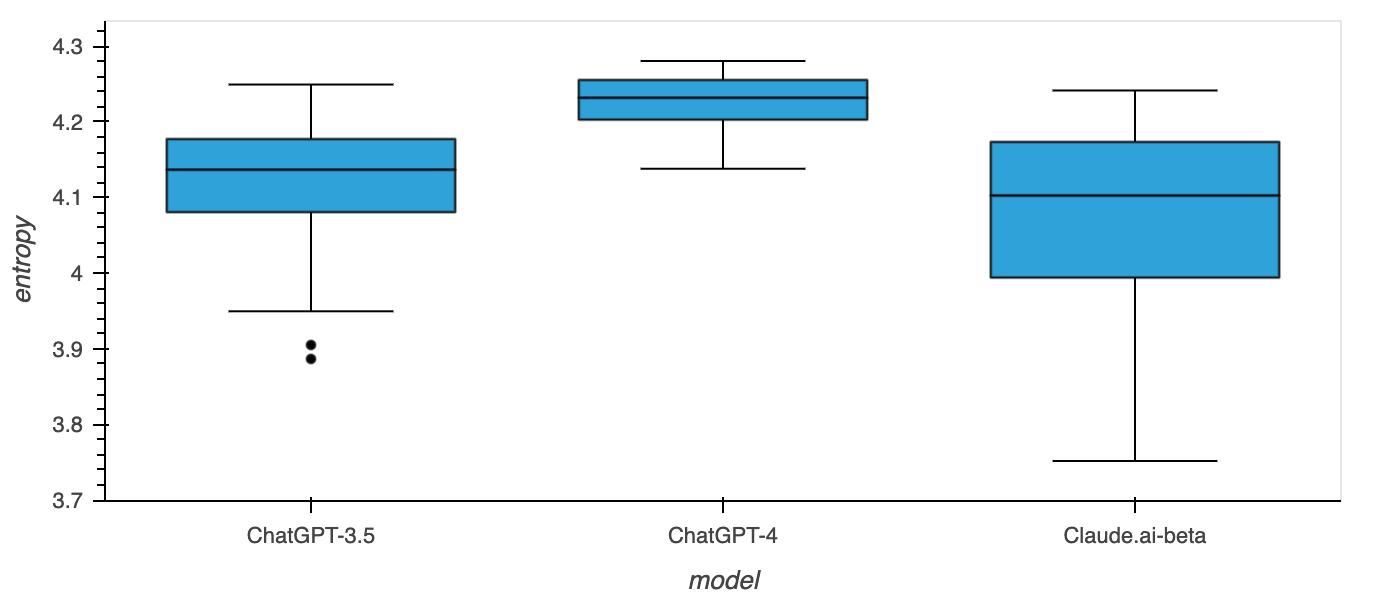
\includegraphics[width=11.5cm]{Figures/fig19.png}
\end{figure}
\end{frame}


\begin{frame}{Entropy Of Policy Relation 3, Among Paradigms}
\begin{figure}[H]
% \caption{Economy Category}
\centering
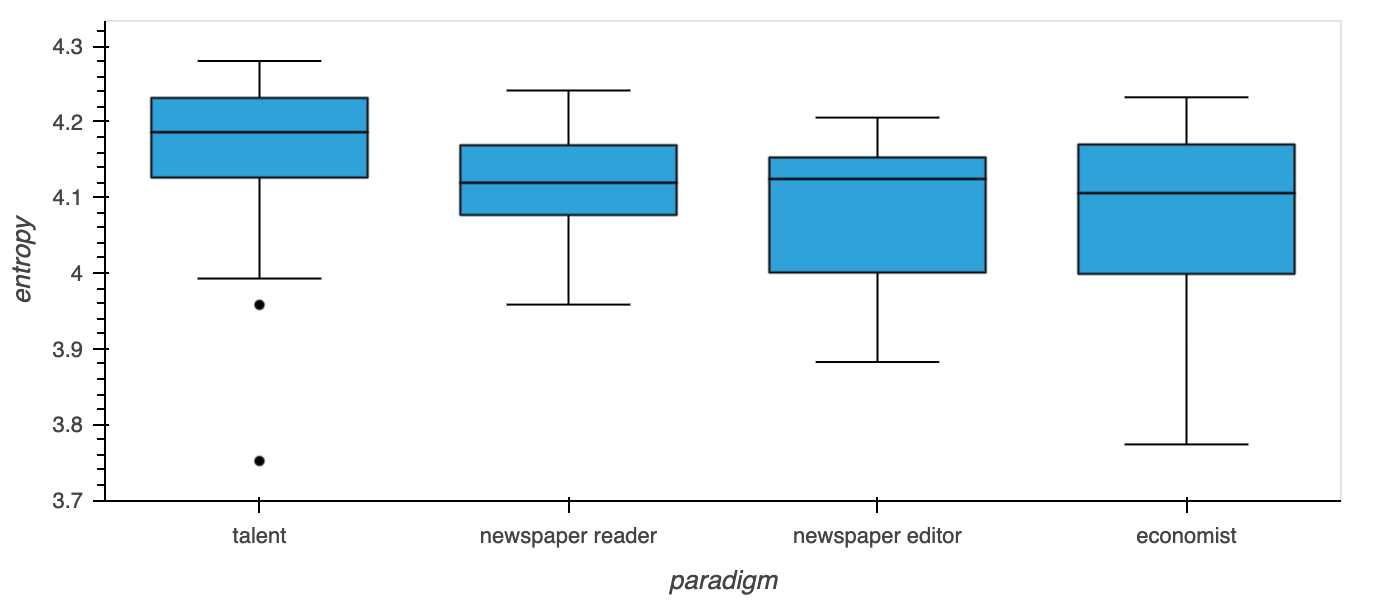
\includegraphics[width=11.5cm]{Figures/fig20.png}
\end{figure}
\end{frame}


\begin{frame}{Entropy Of Policy Relation 4, Among Models}
\begin{figure}[H]
% \caption{Economy Category}
\centering
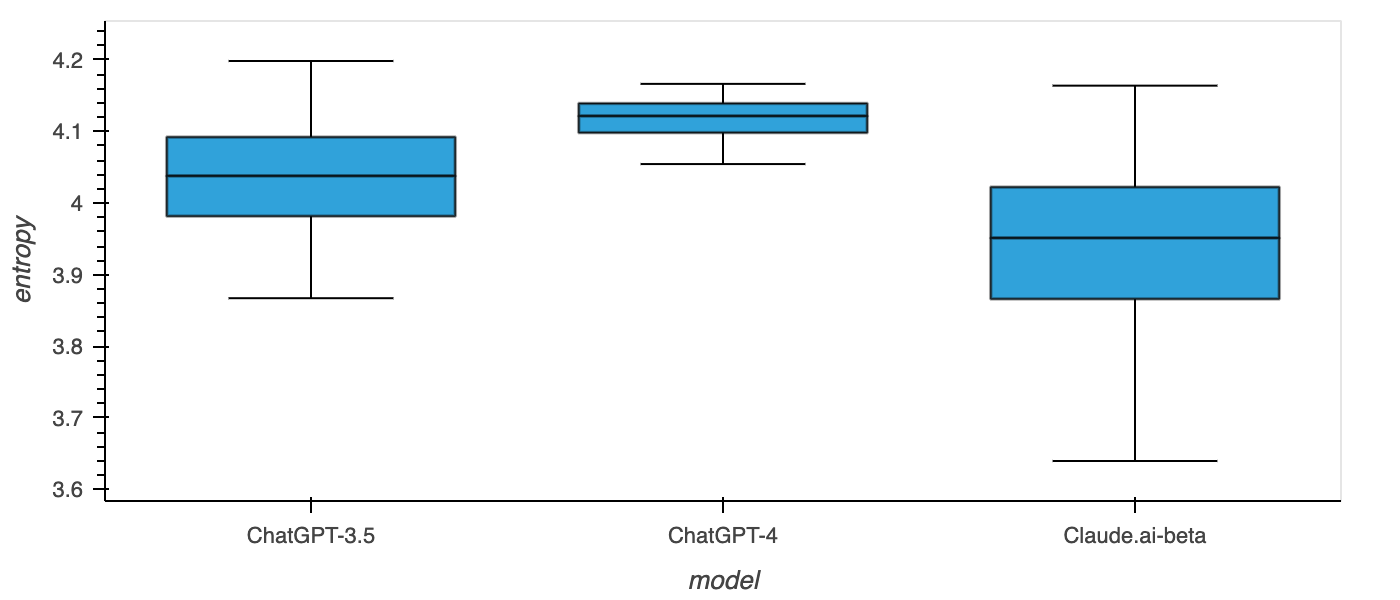
\includegraphics[width=11.5cm]{Figures/fig21.png}
\end{figure}
\end{frame}


\begin{frame}{Entropy Of Policy Relation 4, Among Paradigms}
\begin{figure}[H]
% \caption{Economy Category}
\centering
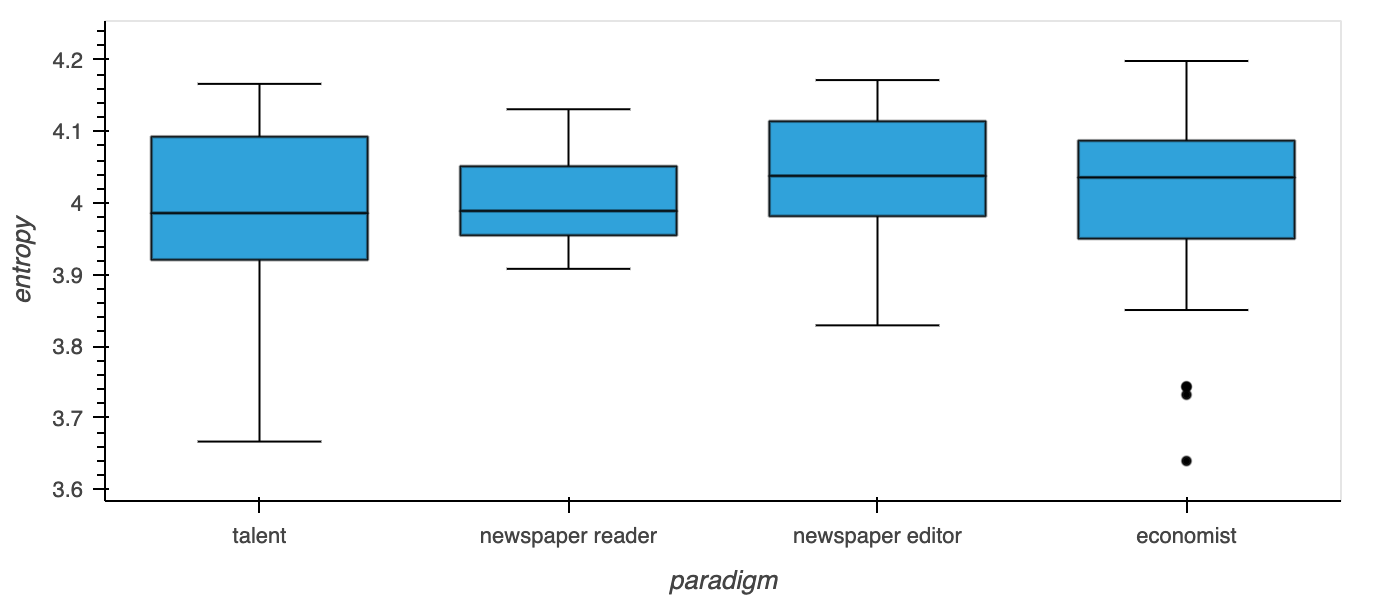
\includegraphics[width=11.5cm]{Figures/fig22.png}
\end{figure}
\end{frame}


\subsection{Similarity}
\begin{frame}{Policy Similarity Among Models}
\begin{figure}[H]
% \caption{Economy Category}
\centering
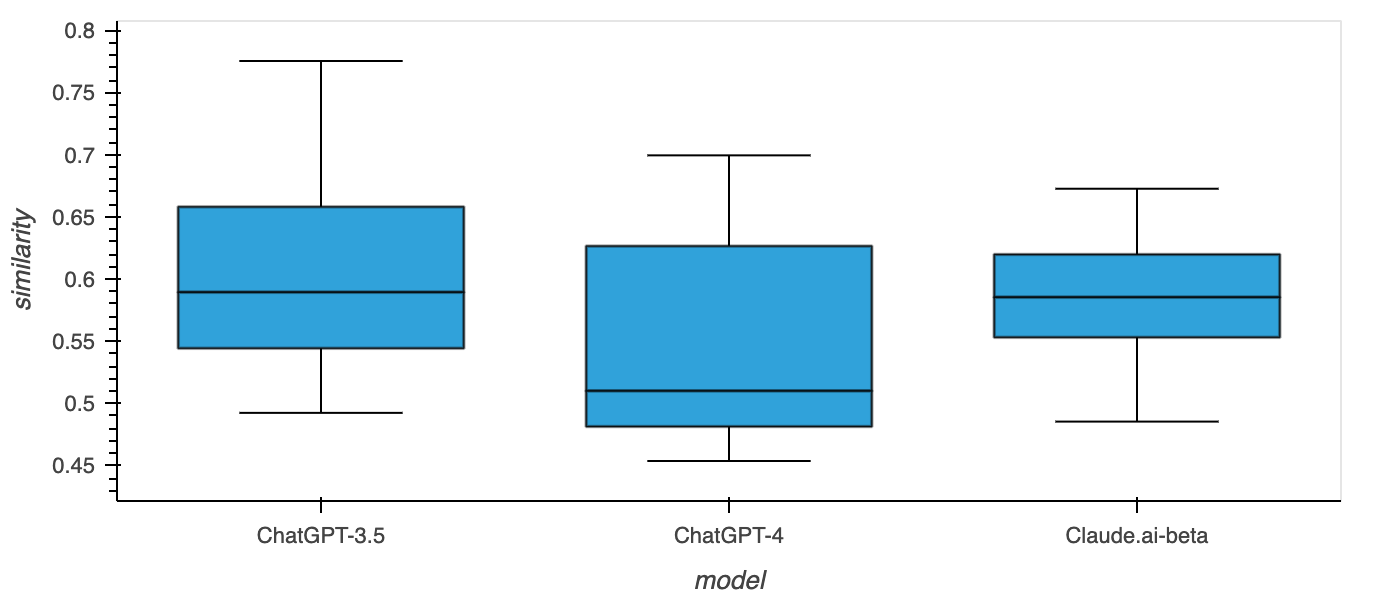
\includegraphics[width=11.5cm]{Figures/fig23.png}
\end{figure}
\end{frame}


\begin{frame}{Policy Similarity Among Paradigms}
\begin{figure}[H]
% \caption{Economy Category}
\centering
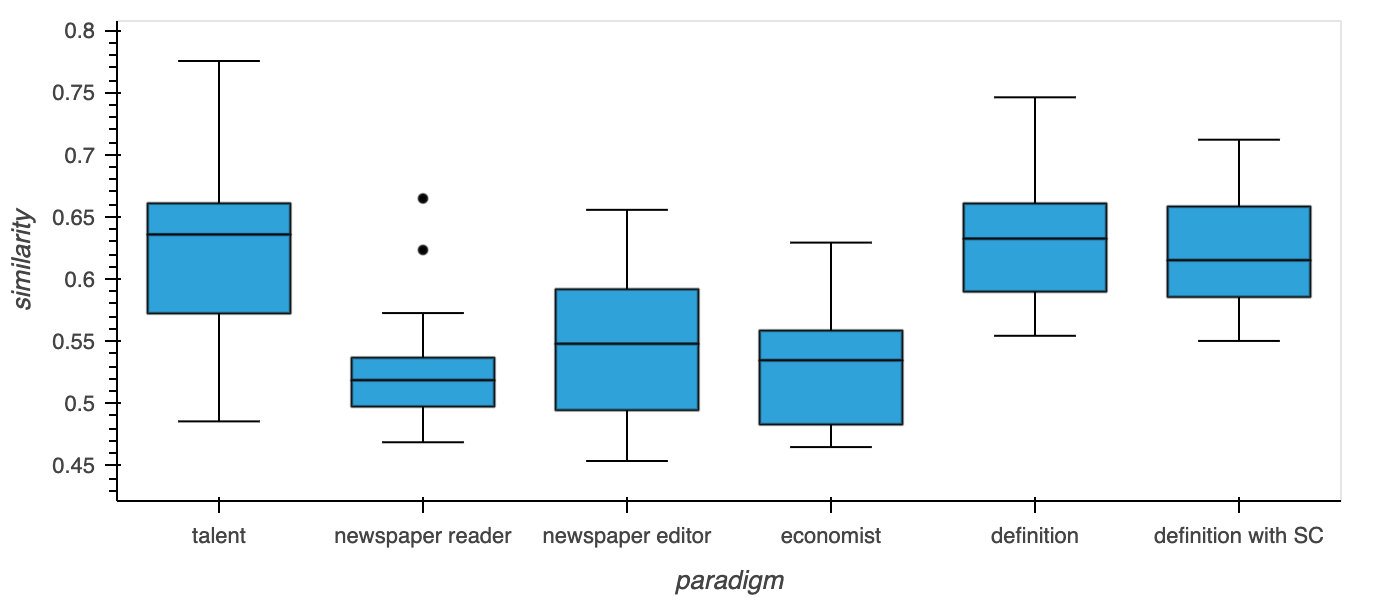
\includegraphics[width=11.5cm]{Figures/fig24.png}
\end{figure}
\end{frame}


\begin{frame}{Uncertainty Similarity Among Models}
\begin{figure}[H]
% \caption{Economy Category}
\centering
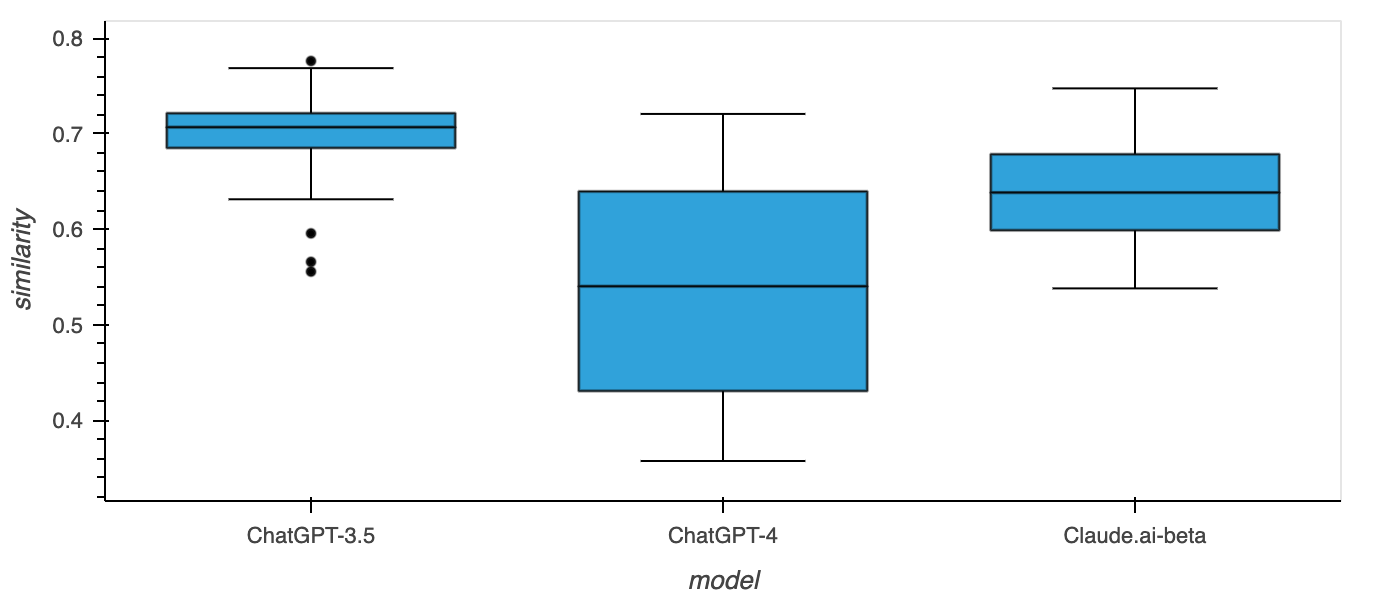
\includegraphics[width=11.5cm]{Figures/fig25.png}
\end{figure}
\end{frame}


\begin{frame}{Uncertainty Similarity Among Paradigms}
\begin{figure}[H]
% \caption{Economy Category}
\centering
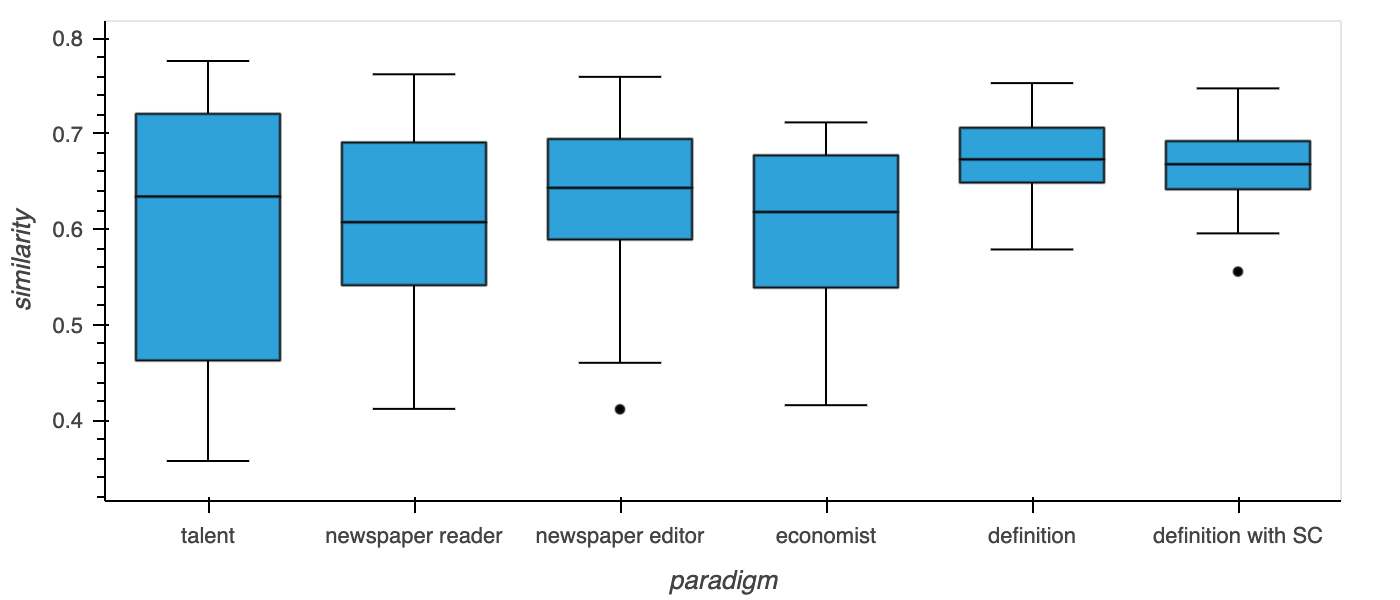
\includegraphics[width=11.5cm]{Figures/fig26.png}
\end{figure}
\end{frame}


\begin{frame}{Uncertainty Similarity Among Models}
\begin{figure}[H]
% \caption{Economy Category}
\centering
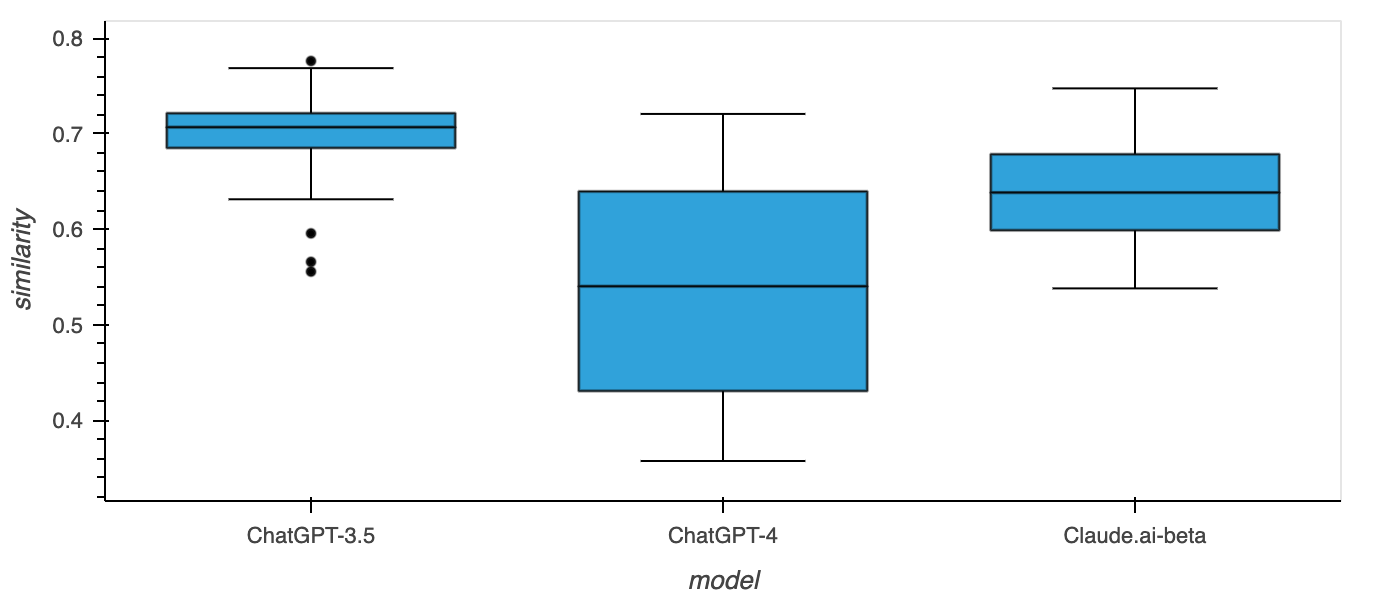
\includegraphics[width=11.5cm]{Figures/fig25.png}
\end{figure}
\end{frame}


\begin{frame}{Uncertainty Similarity Among Paradigms}
\begin{figure}[H]
% \caption{Economy Category}
\centering
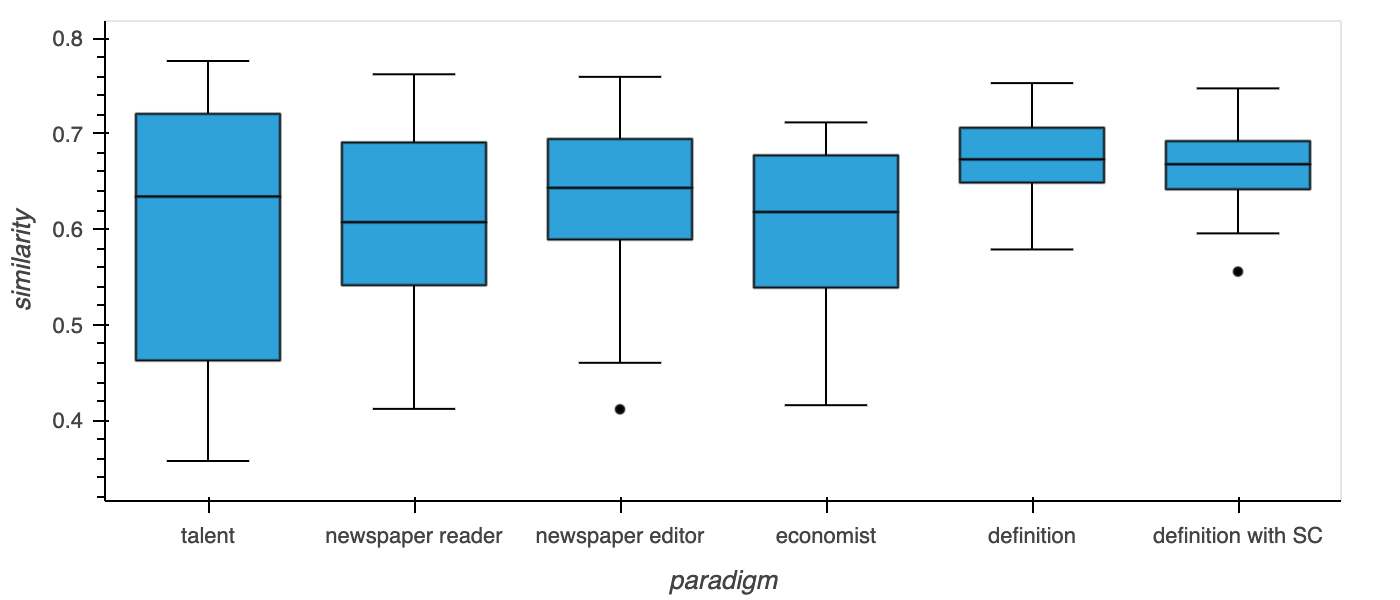
\includegraphics[width=11.5cm]{Figures/fig26.png}
\end{figure}
\end{frame}


\begin{frame}{Similarity Of Policy Relation 1 Among Models}
\begin{figure}[H]
% \caption{Economy Category}
\centering
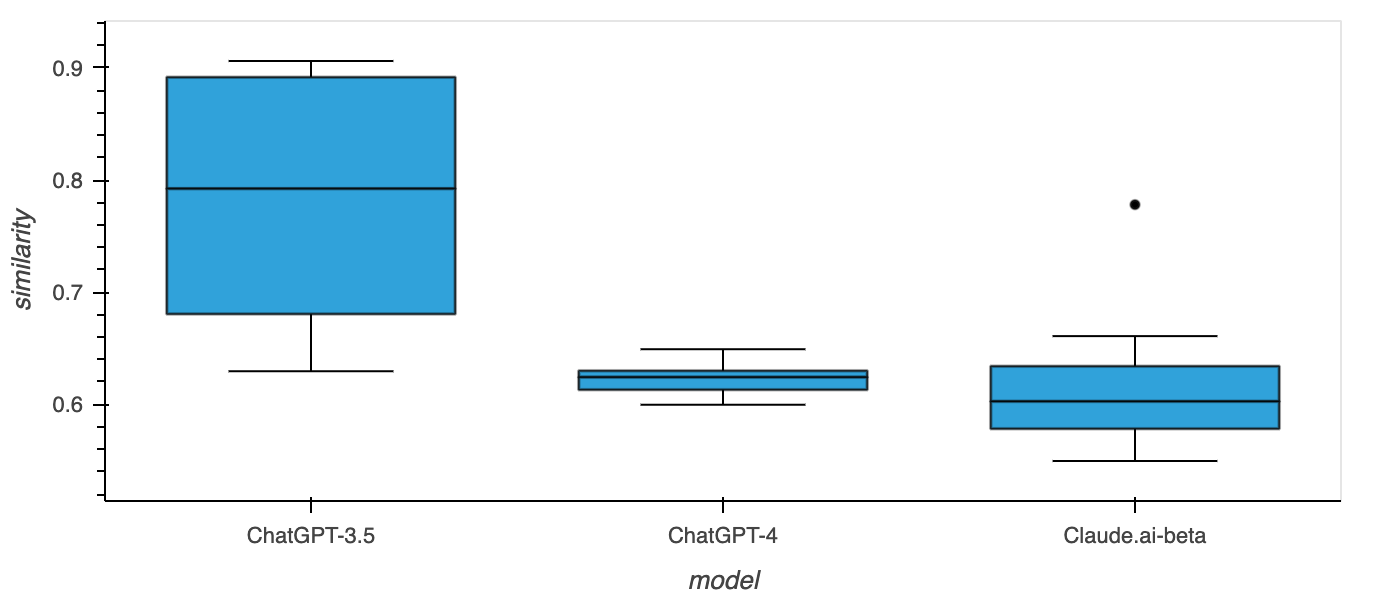
\includegraphics[width=11.5cm]{Figures/fig27.png}
\end{figure}
\end{frame}


\begin{frame}{Similarity Of Policy Relation 1 Among Paradigms}
\begin{figure}[H]
% \caption{Economy Category}
\centering
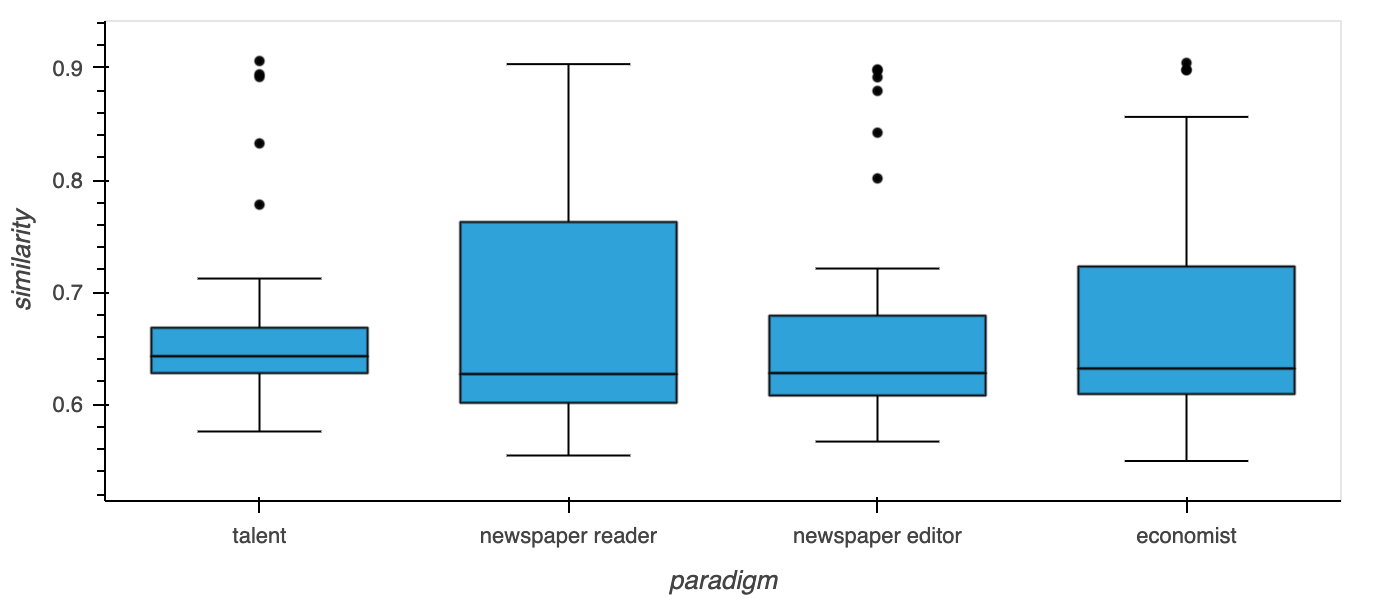
\includegraphics[width=11.5cm]{Figures/fig28.png}
\end{figure}
\end{frame}


\begin{frame}{Similarity Of Policy Relation 2 Among Models}
\begin{figure}[H]
% \caption{Economy Category}
\centering
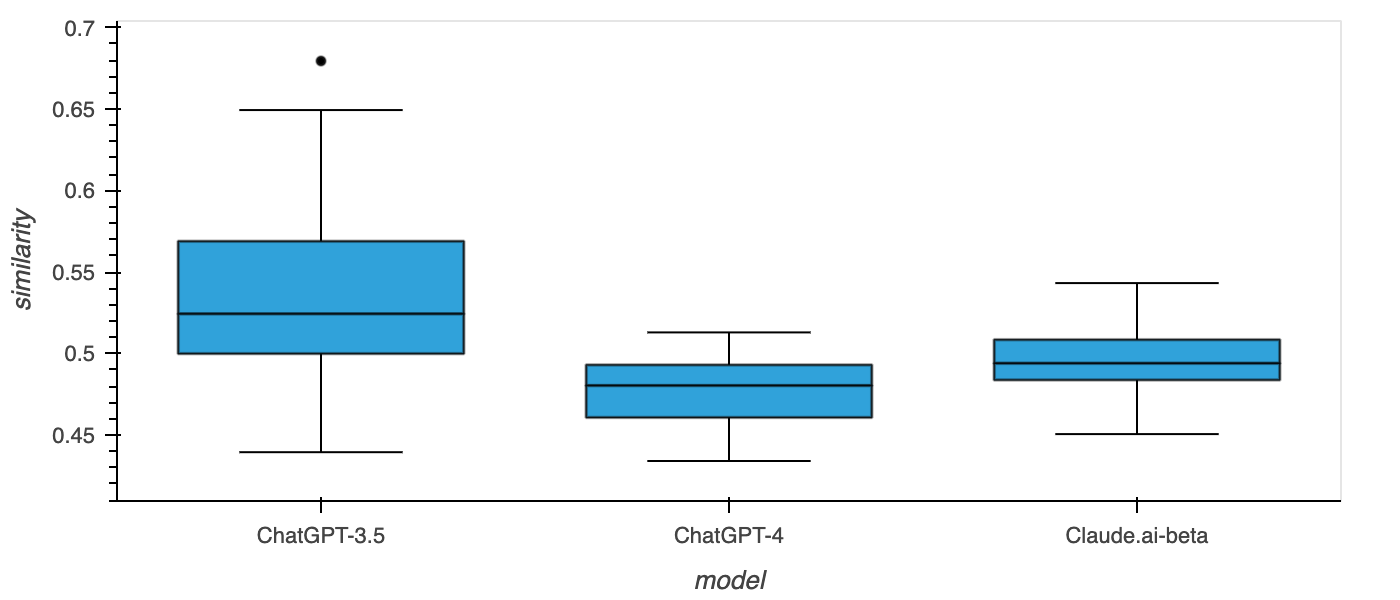
\includegraphics[width=11.5cm]{Figures/fig29.png}
\end{figure}
\end{frame}


\begin{frame}{Similarity Of Policy Relation 2 Among Paradigms}
\begin{figure}[H]
% \caption{Economy Category}
\centering
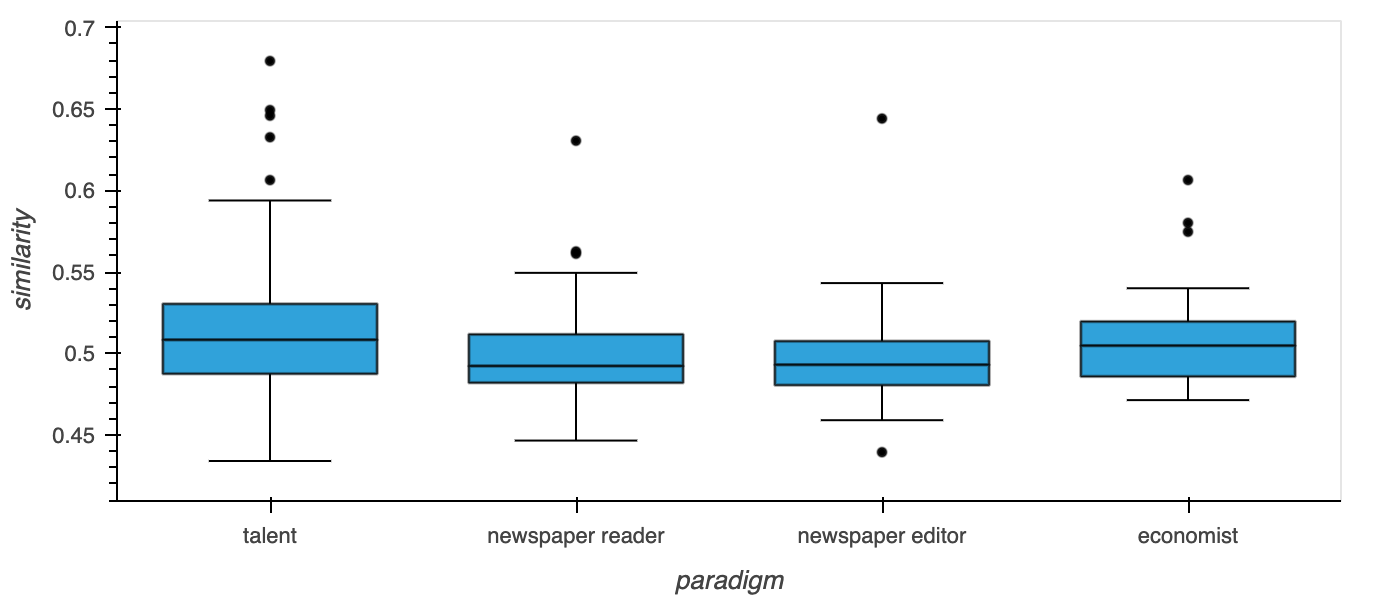
\includegraphics[width=11.5cm]{Figures/fig30.png}
\end{figure}
\end{frame}


\begin{frame}{Similarity Of Policy Relation 3 Among Models}
\begin{figure}[H]
% \caption{Economy Category}
\centering
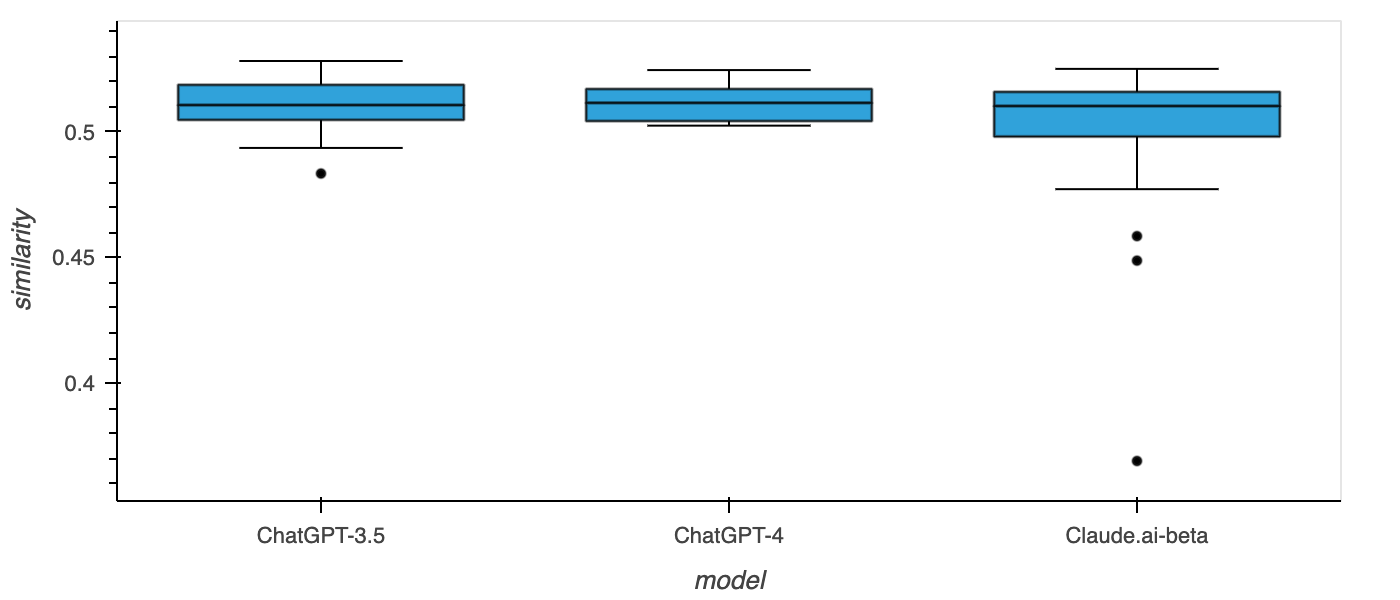
\includegraphics[width=11.5cm]{Figures/fig31.png}
\end{figure}
\end{frame}


\begin{frame}{Similarity Of Policy Relation 3 Among Paradigms}
\begin{figure}[H]
% \caption{Economy Category}
\centering
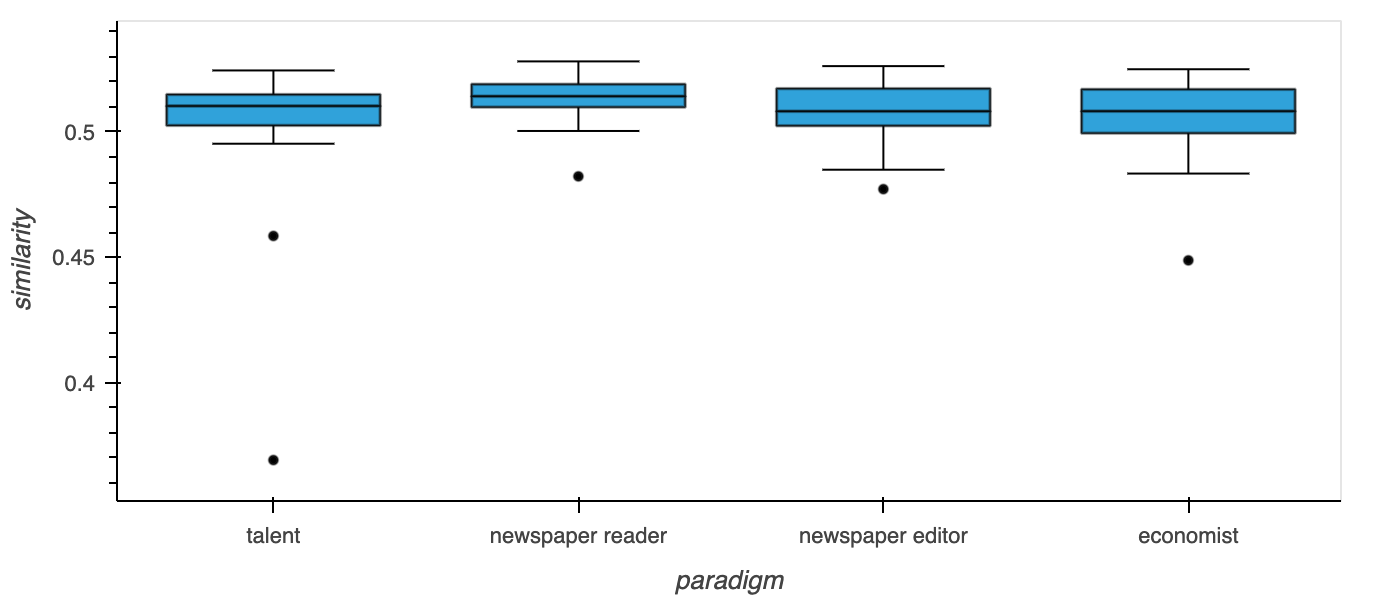
\includegraphics[width=11.5cm]{Figures/fig32.png}
\end{figure}
\end{frame}


\begin{frame}{Similarity Of Policy Relation 4 Among Models}
\begin{figure}[H]
% \caption{Economy Category}
\centering
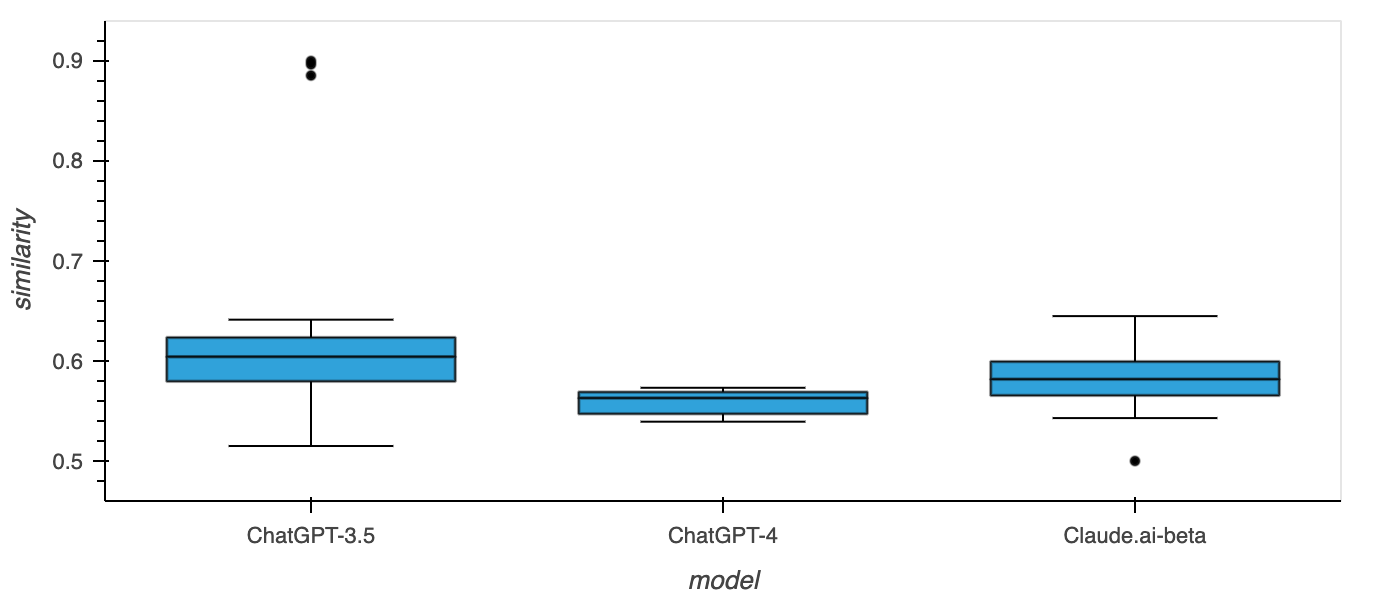
\includegraphics[width=11.5cm]{Figures/fig33.png}
\end{figure}
\end{frame}


\begin{frame}{Similarity Of Policy Relation 4 Among Paradigms}
\begin{figure}[H]
% \caption{Economy Category}
\centering
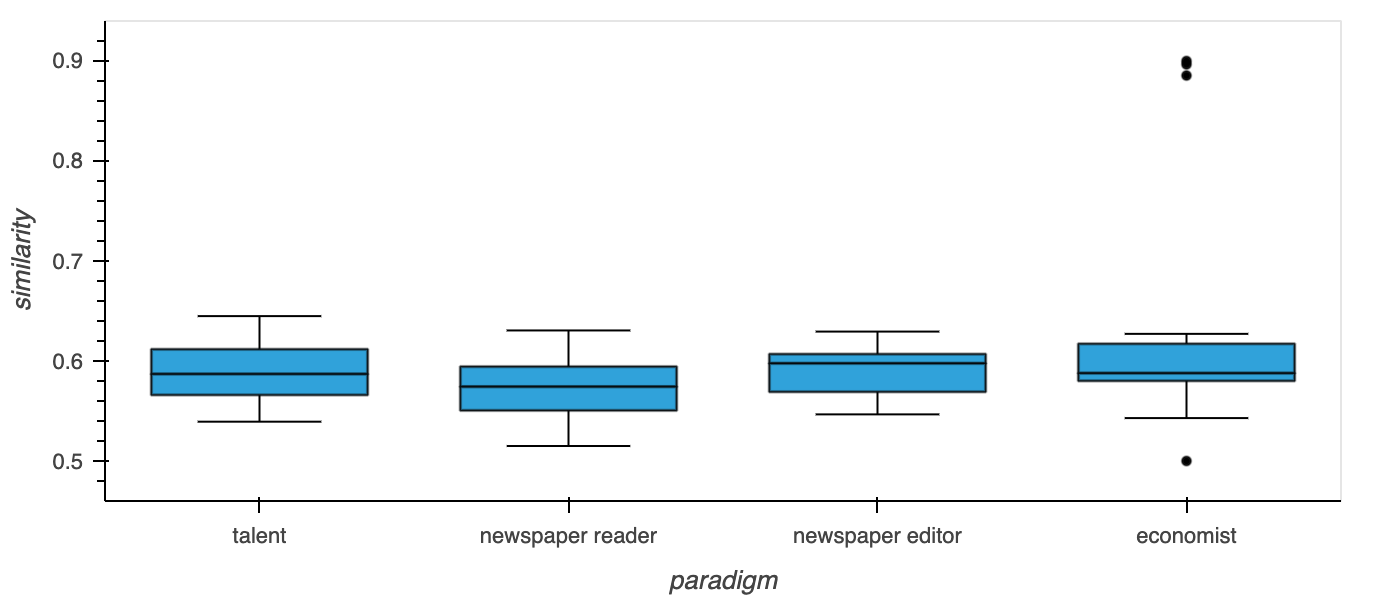
\includegraphics[width=11.5cm]{Figures/fig34.png}
\end{figure}
\end{frame}


\begin{frame}{Country-Level Comprehension, Literature}
\begin{itemize}
    \item Taiwan LLM
    \item LLM-Eval
\end{itemize}
\end{frame}


\section{References}


\begin{frame}[allowframebreaks]{}
\renewcommand{\section}[2]{}%
\bibliography{/Users/jackyyeh/Library/texmf/bibtex/bib/Zotero.bib}
\end{frame}
\end{document}
